\let\negmedspace\undefined
\let\negthickspace\undefined
\documentclass[journal]{IEEEtran}
\usepackage[a5paper, margin=10mm, onecolumn]{geometry}
%\usepackage{lmodern} % Ensure lmodern is loaded for pdflatex
\usepackage{tfrupee} % Include tfrupee package

\setlength{\headheight}{1cm} % Set the height of the header box
\setlength{\headsep}{0mm}     % Set the distance between the header box and the top of the text

\usepackage{gvv-book}
\usepackage{gvv}
\usepackage{cite}
\usepackage{amsmath,amssymb,amsfonts,amsthm}
\usepackage{algorithmic}
\usepackage{graphicx}
\usepackage{textcomp}
\usepackage{xcolor}
\usepackage{txfonts}
\usepackage{listings}
\usepackage{enumitem}
\usepackage{mathtools}
\usepackage{gensymb}
\usepackage{comment}
\usepackage[breaklinks=true]{hyperref}
\usepackage{tkz-euclide} 
\usepackage{listings}
% \usepackage{gvv}                                        
\def\inputGnumericTable{}                                 
\usepackage[latin1]{inputenc}                                
\usepackage{color}                                            
\usepackage{array}                                            
\usepackage{longtable}                                       
\usepackage{calc}                                             
\usepackage{multirow} 
\usepackage{hhline}                                           
\usepackage{ifthen}                                           
\usepackage{lscape}
\usepackage{circuitikz}
\tikzstyle{block} = [rectangle, draw, fill=blue!20, 
    text width=4em, text centered, rounded corners, minimum height=3em]
\tikzstyle{sum} = [draw, fill=blue!10, circle, minimum size=1cm, node distance=1.5cm]
\tikzstyle{input} = [coordinate]
\tikzstyle{output} = [coordinate]

\begin{document}
\bibliographystyle{IEEEtran}
\vspace{3cm}

\title{MatGeo Assignment 4.12.12}
\author{AI25BTECH11007}
 \maketitle
% \newpage
% \bigskip
{\let\newpage\relax\maketitle}

\renewcommand{\thefigure}{\theenumi}
\renewcommand{\thetable}{\theenumi}
\setlength{\intextsep}{10pt} % Space between text and floats


\numberwithin{equation}{enumi}
\numberwithin{figure}{enumi}
\renewcommand{\thetable}{\theenumi}
\noindent
\textbf{Question:}\\
For what values of a and b the intercepts cut off on the coordinate axes by the line ax+by+8 = 0 are equal in length but opposite in signs to those cut off by the line 2x-3y = 0 on the axes.

\noindent\\
\textbf{Solution:}\\
\[
\text{Line : } ax+by+8=0 
\quad\Longleftrightarrow\quad 
\myvec{a & b} \myvec{x \\ y} + 8 = 0
\]
         
\[
\text{Intercept vector: }
\myvec{-\tfrac{8}{a} \\[2mm] -\tfrac{8}{b}}
\]

\[
\text{For } 2x-3y=0 \;\;\Longleftrightarrow\;\; 
\frac{x}{3}+\frac{y}{-2}=0,
\quad
\text{intercept vector: }
\myvec{3 \\ -2}
\]

\[
\text{Condition: }\;
\myvec{-\tfrac{8}{a} \\[2mm] -\tfrac{8}{b}}
=
-\myvec{3 \\ -2}
\]

\[
\Rightarrow\quad 
-\frac{8}{a} = -3, 
\quad 
-\frac{8}{b} = 2
\]

\[
\Rightarrow\quad 
a = \tfrac{8}{3}, 
\quad 
b = -4
\]

\begin{figure}
    \centering
    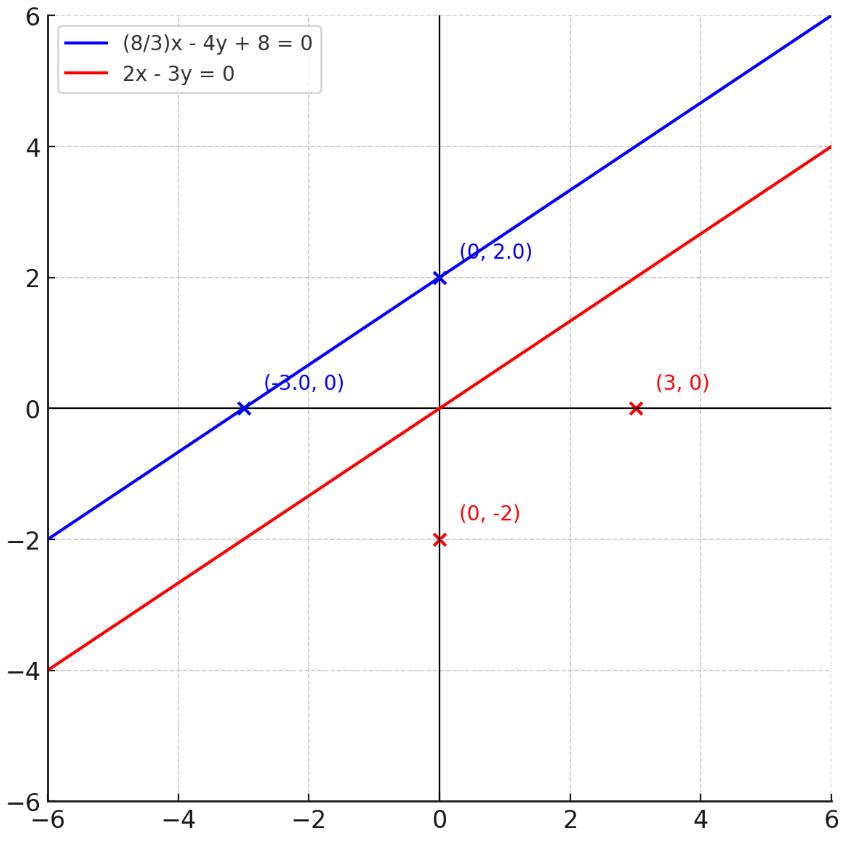
\includegraphics[width=0.75\linewidth]{figs/image.png}
    \caption{Plot}
    \label{fig:placeholder}
\end{figure}
\end{document}